\subsection{Prestazioni}

A conclusione di tale capitolo vengono riportate le prestazioni del DDPM implementato da Ho et al.~\cite{ho2020},
misurate ricorrendo a due notorie metriche, ampiamente usate in letteratura, per valutare la qualità delle immagini prodotte da modelli generativi. 
Entrambe le due suddette metriche si avvalgono di una rete \emph{Inception-v3}~\cite{szegedyRethinkingInceptionArchitecture2015}, 
un classificatore di immagini pre-addestrato su ImageNet\footnote{\url{https://www.image-net.org/}}. In particolare:
\begin{itemize}
\item la metrica IS (\emph{Inception Score}) valuta la sola distribuzione delle immagini generate dal modello: 
ad un punteggio IS elevato corrisponde una migliore \emph{qualità} e \emph{varietà} delle immagini generate dal modello. 
\item la metrica FID (\emph{Fréchet Inception Distance}) confronta le distribuzioni delle immagini generate dal modello con quelle 
delle immagini del dataset di addestramento. Tale metrica, dal momento che “\emph{cattura la somiglianza delle immagini generate con quelle reali, 
meglio di quanto non faccia la metrica IS}”~\cite{heuselGANsTrainedTwo2017}, è lo standard \emph{de facto} per valutare la qualità delle immagini prodotte dai modelli generativi. 
Più basso è il il punteggio FID, più la distribuzione delle immagini generate si avvicina alla distribuzione delle immagini del dataset di addestramento.
\end{itemize}

\noindent Come già accennato in precedenza, Ho et al.~\cite{ho2020} hanno scelto $T=1000$ e hanno propeso, nel processo di diffusione in avanti, 
per uno schema di diffusione \emph{lineare}, con i $\beta_t$ che si incrementano linearmente da $\beta_1 = 10^{-4}$ a $\beta_T=0.02$. 
Gli iperparametri $\beta_t$, che implementano lo schema di diffusione, sono stati scelti molto più piccoli rispetto ai valori dei pixel delle immagini
di addestramento normalizzati tra $[-1, 1]$, cosicché le transizioni delle catene markoviane dei processi di diffusione diretta e inversa 
esibiscano approssimativamente la medesima forma funzionale (distribuzione gaussiana)
mantenendo, al contempo, il rapporto segnale rumore a valle della diffusione in avanti, il più contenuto possibile
($L_T=D_{KL}(q(\mathbf{x}_T|\mathbf{x}_0)\,\|\,\mathcal{N}(\bm{0},\bm{I})) \approx 10^{-5}$ bit per dimensione~\cite{ho2020}).

\noindent
Come si evince dalla Figura~\ref{fig:performance}, con un punteggio FID\footnote{i punteggi IS e FID riportati in Figura~\ref{fig:performance} sono stati calcolati su $50000$ campioni del dataset di addestramento CIFAR-10.} di $3.17$, 
il modello incondizionato addestrato da Ho et al.~\cite{ho2020} sul dataset CIFAR-10\footnote{Il dataset CIFAR-10 consiste di $60000$ immagini $32\times32$ a colori suddivise in 
$10$ classi, con $6000$ immagini per classe. Tale dataset annovera $50000$ immagini per l'addestramento e $10000$ per la fase di testing.} 
ottiene una migliore qualità dei campioni rispetto alla maggior parte dei modelli in letteratura, inclusa la classe dei modelli condizionali.



\begin{figure}[tp]
\centering
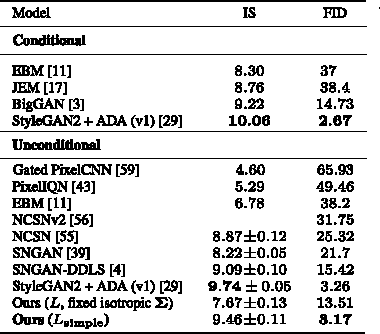
\includegraphics[keepaspectratio,scale=1.2]{performance.pdf}
\caption{Prestazioni DDPM. Fonte~\cite{ho2020}}\label{fig:performance}
\end{figure}